\documentclass[10pt]{article}

\usepackage[T1]{fontenc}
\usepackage[utf8]{inputenc}
%\usepackage{beton}
%\usepackage{ccfonts}
%\usepackage{concrete}
\usepackage{concmath}
\usepackage{eulervm}
\usepackage{amsmath,amsthm,amssymb}
\usepackage{mathtools}
\usepackage{multicol}
\usepackage{marginnote}
\usepackage{pgfplots}
\usepackage{float}
\usepackage{hyperref}
\usepackage{bbm}
\usepackage{booktabs}
\pgfplotsset{compat=1.5}

\usepackage{listings}
\usepackage{xcolor}
\definecolor{codegreen}{rgb}{0,0.6,0}
\definecolor{codegray}{rgb}{0.5,0.5,0.5}
\definecolor{codepurple}{rgb}{0.58,0,0.82}
\definecolor{backcolour}{rgb}{0.95,0.95,0.92}
\lstdefinestyle{mystyle}{
    backgroundcolor=\color{backcolour},   
    commentstyle=\color{codegreen},
    keywordstyle=\color{magenta},
    numberstyle=\tiny\color{codegray},
    stringstyle=\color{codepurple},
    basicstyle=\ttfamily\footnotesize,
    breakatwhitespace=false,         
    breaklines=true,                 
    captionpos=b,                    
    keepspaces=true,                 
    numbers=left,                    
    numbersep=5pt,                  
    showspaces=false,                
    showstringspaces=false,
    showtabs=false,                  
    tabsize=2
}

\lstset{language=Python, style=mystyle}

\usepackage{mathtools}

\usepackage{wasysym}
\usepackage[margin=1.5in]{geometry} 
\usepackage{enumerate}
\index{\usepackage}\usepackage{multicol}

\newcommand{\N}{\mathbf{N}}
\newcommand{\Z}{\mathbb{Z}}

\newcommand{\R}{\mathbf{R}}
\newcommand{\C}{\mathbf{C}}
\newcommand{\Pbb}{\mathbb{P}}
\newcommand{\Fcal}{\mathcal{F}}
\newcommand{\Lcal}{\mathcal{L}}
\newcommand{\Acal}{\mathcal{A}}
\newcommand{\Ecal}{\mathcal{E}}
\newcommand{\Ebb}{\mathbb{E}}
\newcommand{\Qbb}{\mathbb{Q}}


\renewcommand{\mathbf}{\mathbold}

\newenvironment{theorem}[2][Theorem]{\begin{trivlist}
  \item[\hskip \labelsep {\bfseries #1}\hskip \labelsep {\bfseries #2.}]}{\end{trivlist}}
\newenvironment{lemma}[2][Lemma]{\begin{trivlist}
  \item[\hskip \labelsep {\bfseries #1}\hskip \labelsep {\bfseries #2.}]}{\end{trivlist}}
\newenvironment{exercise}[2][Exercise]{\begin{trivlist}
  \item[\hskip \labelsep {\bfseries #1}\hskip \labelsep {\bfseries #2.}]}{\end{trivlist}}
\newenvironment{reflection}[2][Reflection]{\begin{trivlist}
  \item[\hskip \labelsep {\bfseries #1}\hskip \labelsep {\bfseries #2.}]}{\end{trivlist}}
\newenvironment{proposition}[2][Proposition]{\begin{trivlist}
  \item[\hskip \labelsep {\bfseries #1}\hskip \labelsep {\bfseries #2.}]}{\end{trivlist}}
\newenvironment{corollary}[2][Corollary]{\begin{trivlist}
  \item[\hskip \labelsep {\bfseries #1}\hskip \labelsep {\bfseries #2.}]}{\end{trivlist}}

\newenvironment{definition}[2][Definition]{\begin{trivlist}
  \item[\hskip \labelsep {\bfseries #1}\hskip \labelsep {\bfseries #2.}]}{\end{trivlist}}

\begin{document}
	
  
  \renewcommand{\qedsymbol}{\blacksquare}
	\title{Investments Class \\ Problem set 3}
	\author{Daniel Grosu, William Martin, Denis Steffen}
	
	\maketitle

  \begin{exercise}{1}(Efficient portfolios)
    \begin{itemize}
      \item
    The return on the portfolio is linear in the returns of the risky assets and
    the risk-free return:
    \begin{align*}
      \mu_P &= \mu^T \omega + (1 - \mathbbm{1}^T \omega) R_f \\
      \mu_P - R_f &= \mu^T \omega +  - \mathbbm{1}^T \omega R_f \\
      \mu_P - R_f &= (\mu - R_f\mathbbm{1})^T \omega
    \end{align*}
    where $\mathbbm{1}$ is the $N \times 1$ vector of ones. The maximization is
    then formulated in terms of the Lagrangian with no constraints:
    \begin{align*}
      \Lcal = (R_f + (\mu - \mathbbm{1}R_f)^T \omega) - \gamma \frac 1 2 \omega^T \Sigma \omega.
    \end{align*}
    The FOC condition with respect to $\omega$ reads as:
    \begin{align*}
      \frac{\partial \Lcal}{\partial \omega} = \mu - \mathbbm{1} R_f - \gamma \Sigma \omega = 0
    \end{align*}
    and solving for $\omega$ yields the following optimal $\omega^*$:
    \begin{align*}
      \omega^* = \gamma^{-1}\Sigma^{-1} \left( \mu - R_f \mathbbm{1} \right)
    \end{align*}
    The $\omega^*$ is optimal since the Hessian $\frac{\partial^2
      \Lcal}{\partial \omega\partial \omega^\top} = -\Sigma$ is negative semi-definite.
      \begin{align*}
        cov \left[R, R_p \right] &= cov \left[ R, R_f + (\omega^*)^T(R - R_f\mathbbm{1}) \right] \\
        &= cov \left[ R, (\omega^*)^T R \right]a \\
        &= cov \left[ R - \mu, R - \mu \right] \omega^* \\
        &= var \left[ R, R \right] \omega^* \\
        &= \Sigma \omega^* \\
        &= \Sigma \gamma^{-1} \Sigma^{-1} (\mu - R_f \mathbbm{1}) \\
        &=\gamma^{-1}(\mu - R_f \mathbbm{1}) \\
        &\Downarrow \\
          \gamma cov\left[ R, R_p \right]&= \mu - R_f\mathbbm{1} \;\;\; (\star)
      \end{align*}
      \item
        Using the definition of $\mu_P$ and the previously proven identity, it
        follows that
        \begin{align*}
          \mu_P = \Ebb\left[ R_p \right] &= \Ebb\left[ R_f + \omega^T(R - R_f\mathbbm{1}) \right] \\
          &= R_f + \omega^T ( \mu - R_f \mathbbm{1}) \\                                         &= \omega^T \mu + (1 - \omega^T \mathbbm{1}) R_f \\
          &= \omega^T(\mu - \mathbbm{1}R_f) + R_f \\
          &\stackrel{\star}{=} \omega^T\gamma cov\left[ R, R_p \right] + R_f \\
          &= \gamma cov \left[ \omega^TR, R_p \right]+ R_f \\
          &= \gamma cov \left[ R_p, R_p \right] + R_f\\
          &= \gamma \sigma^2_P  + R_f\\
          &\Downarrow \\
          \mu_P - R_f &= \gamma \sigma_P^2\\
          &\Downarrow \\
          \gamma &= \frac{\mu_P - R_f}{\sigma_P^2}\\
          & \Downarrow \\
          (\mu - R_f \mathbbm{1}) &\stackrel{\star}{=} \gamma cov\left[ R, R_p \right] = \frac{cov\left[ R, R_p \right]}{\sigma_P^2} (\mu_P - R_f) = \beta_{P} (\mu_P - R_f) \;\;\; (\star \star)
          \end{align*}
          Where $\beta_{P} = (\beta_{1, P}, \ldots, \beta_{N, P})^T$.

          \item
            A linear regression model is
            \begin{align*}
              Y = X_1 \beta_1 + \cdots + X_N \beta_N + \epsilon
            \end{align*}
            with the following assumptions:
            \begin{enumerate}[\textbf{A}1.]
              \item \textbf{Linearity} between $Y$ and $X_i$.
              \item \textbf{Full rank}  of $X$.
              \item \textbf{Exogeneity}: $\Ebb\left[ \epsilon \mid X_1,
                  \cdots, X_ \right] = 0$.
              \item \textbf{Homoskedasticity and nonautocorrelation}: 
                $cov(\epsilon_i, \epsilon_j | X_i, X_j) = 0 \;\; \forall i \neq j$
                and $var(\epsilon_i \mid X_1, \ldots, X_N) = \sigma^2$.
              \item \textbf{Normality of the errors}: $\epsilon \mid X_1,
                \ldots, X_N \sim N(0, \sigma^2)$.
            \end{enumerate}

            The above assumptions are satisfied when regressing the excess
            return of an asset on the excess return of the market portfolio:

            \begin{align*}
              R_i &= R_f + \beta_i(R_P - R_f) + \epsilon_i \\
              R_i - R_f &= \beta_i(R_P - R_f) + \epsilon_i
            \end{align*}

            The exogeneity assumption is verified by taking the expectation of
            the model:

            \begin{align*}
              \Ebb\left[ R_i - R_f \right] &= \beta_i \Ebb\left[ R_P - R_f \right] + \Ebb\left[ \epsilon_i \right] \\
              \mu_i - R_f &= \beta_i (\mu_P - R_f) + \Ebb\left[ \epsilon_i \right] \\
               0 &\stackrel{\star \star}{=} \Ebb\left[ \epsilon_i \right]
            \end{align*}

            To check the homoskedasticity assumption, take the covariance of each side of
            the model with the stochastic return on the market
            portfolio:

            \begin{align*}
              cov(R_i - R_f, R_P) &= \beta_icov(R_p - R_f, R_P) + cov(\epsilon_i, R_p) \\
              cov(R_i, R_P) &= \beta_icov(R_P, R_P) + cov(\epsilon_i, R_p) \\
              cov(R_i, R_P) &= \frac{cov(R_i, R_P)}{\sigma_P^2}cov(R_P, R_P) + cov(\epsilon_i, R_p) \\
              cov(\epsilon_i, R_p) &= 0
            \end{align*}

            The previously found expression for $\beta_{i, P}$ is consistent:
            \begin{align*}
              \beta_{i} = \frac{cov(R_i - R_f, R_P - R_f)}{var(R_P - R_f)} = \frac{cov(R_i, R_P)}{\sigma_P^2} = \beta_{i, P}
              \end{align*}
              When regressing on $R_i$ alone and not on the excess above $R_f$, the intersect is still
              $R_f$ as it follows from the previously found identity and the
              fact that $\Ebb\left[ \epsilon_i \right] = 0$.
            \item
              \begin{proposition}{[Sharpe-Ratios]}
              All the mean-variance efficient portfolios have the same Sharpe
              ratio where we define its Sharpe ratio as $SR_p = \frac{\mu_p -
                R_f}{\sigma_P}$:
              \end{proposition}
              \begin{proof}
              To show that all the portfolios have the same Sharpe ratio we will
              suppose that there exists another portfolio $P'$ and show that
              $SR_P = SR_{P'}$.
              In the previous subtask we found that
              \begin{align*}
                (\mu - R_f \mathbbm{1}) = \beta_P(\mu_P - R_f)
              \end{align*}
              multiplying on the left by the asset weights of the alternative
              mean-variance efficient
              portfolio $\omega_{P'}$ we get that
              \begin{align}
                (\omega_{P'})^T(\mu - R_f \mathbbm{1}) &= (\omega_{P'})^T \frac{cov(R, R_P)}{\sigma_P^2} (\mu_P - R_f) \\
                \label{eq:twoportfolios}
                (\mu_{P'} - R_f) &= \frac{cov(R_{P'}, R_P)}{\sigma_P^2} (\mu_P - R_f)
              \end{align}
              All the mean-variance efficient portfolios are a linear
              combination of the tangent portfolio $R_{tan}$ and the risk-free
              assets $R_f$. Let $\eta$ and $\eta'$ be the weights of the tangent
              portfolio in the portfolios $P$ and $P'$:
              \begin{align*}
                R_{P} &= \eta \times R_{tan} + (1 - \eta) R_f \\
                R_{P'} &= \eta' \times R_{tan} + (1 - \eta') R_f \\
              \end{align*}
              Then the covariance between the two portfolios is
              \begin{align}
                \label{eq:covariances}
                cov(R_P, R_{P'}) = \eta \eta' cov(R_{tan}, R_{tan}) = \eta \eta'
              \end{align}
              while the variances are:
              \begin{align}
                \label{eq:variances}
                \sigma^2_P &= var(R_{P}) = \eta^2 \\
                \sigma^2_{P'} &= var(R_{P'}) = \eta'^2
              \end{align}

              Plugging \autoref{eq:variances} and \autoref{eq:covariances} in
              \autoref{eq:twoportfolios} yields:
              \begin{align*}
                (\mu_{P'} - R_f) &= \frac{\eta \eta'}{\eta^2} (\mu_P - R_f) \\
                \frac{(\mu_{P'} - R_f)}{\eta'} &= \frac{(\mu_P - R_f)}{\eta} \\
                \frac{(\mu_{P'} - R_f)}{\sigma_{P'}} &= \frac{(\mu_P - R_f)}{\sigma_{P}} \\
                SR_{P} &= SR_{P'}
              \end{align*}
              \end{proof}
              
    \end{itemize}
  \end{exercise}

\begin{exercise}{2}(Portfolio math)
   First we show that a convex combination of two minimum variance frontier portfolios $w_a$ and $w_b$ is a minimum variance frontier portfolio.

   $w$ is a minimum variance frontier portfolio if it solves the optimization problem and thus can be written as: 
   $$ w = \lambda\Sigma^{-1}\mathbbm{1}+ \gamma\Sigma^{-1}\mu$$ with $\lambda = \frac{C- \mu_pB}{\Delta}$ and $\gamma = \frac{\mu_pA-B}{\Delta}$. 

   Subsequently consider two arbitrary minimum variance porfolios $w_a$ and $w_b$ with returns $\mu_a$, $\mu_b$ respectively and write $w = \alpha w_a + (1-\alpha)w_b$. 
   Then \begin{align*}
    w &= \alpha (\lambda_a\Sigma^{-1}\mathbbm{1} + \gamma_a\Sigma^{-1}\mu) + (1-\alpha)(\lambda_b\Sigma^{-1}\mathbbm{1} + \gamma_b\Sigma^{-1}\mu) \\
    &= (\alpha \lambda_a + (1-\alpha) \lambda_b)\Sigma^{-1}\mathbbm{1} + (\alpha \gamma_a + (1-\alpha) \gamma_b)\Sigma^{-1}\mu
   \end{align*} 
   But $A,B,C,D$ do not depend on the portfolio but only on the available assets so they do not change between $w_a$ and $w_b$. So we obtain:
   $$ w = \frac{C- (\alpha\mu_a+(1-\alpha)\mu_b)B}{\Delta}\Sigma^{-1}\mathbbm{1} + \frac{(\alpha\mu_p + (1-\alpha)\mu_b)A-B}{\Delta}\Sigma^{-1}\mu$$

  The return of $w$ equals $\alpha\mu_a+(1-\alpha)\mu_b$ and its variance is $\alpha^2 w_a^\top\Sigma w_a + (1-\alpha)^2 w_b^\top\Sigma w_b + 2\alpha(1-\alpha)w_a^\top\Sigma w_b$

  Finally, $w$ is of the form of a minimum variance frontier portfolio solving the following optimization problem: 
  $$ \min_{w} \frac{1}{2} w^\top\Sigma w \text{ such that } w^\top\mu = \alpha\mu_a+(1-\alpha)\mu_b \text{ and } w^\top\mathbbm{1} = 1$$
  
  Conversely, if we have the minimum variance portfolio $w$ and want to write it as a combination of two different portfolios $w_a$ and $w_b$ (with return $\mu_a$ and $\mu_b$), we can define $\alpha = \frac{\mu_p-\mu_b}{\mu_a-\mu_b}, 1- \alpha = \frac{\mu_a - \mu_p}{\mu_a - \mu_b}$. 
  Thus, \begin{align*}
    \alpha w_a + (1-\alpha)w_b &= \frac{C- (\alpha\mu_a+(1-\alpha)\mu_b)B}{\Delta}\Sigma^{-1}\mathbbm{1} + \frac{(\alpha\mu_p + (1-\alpha)\mu_b)A-B}{\Delta}\Sigma^{-1}\mu \\
    &= \frac{C- (\mu_p)B}{\Delta}\Sigma^{-1}\mathbbm{1} + \frac{(\mu_p)A-B}{\Delta}\Sigma^{-1}\mu = w
  \end{align*} because $ \frac{\mu_p-\mu_b}{\mu_a-\mu_b}\mu_a + \frac{\mu_a - \mu_p}{\mu_a - \mu_b}\mu_b = \frac{\mu_p(\mu_a-\mu_b)-\mu_a\mu_b + \mu_a\mu_b}{\mu_a-\mu_b} = \mu_p$
\\
  This proves that any minimum variance frontier portfolio can be replicated by a convex combination of two minimum variance frontier portfolios. 

  For the second part of the exercise, we follow the hint. The expected return of the convex combination of the two portfolios is: $ \Ebb[Y] = wR + (1-w)R_{\text{min}}$. In addition, the variance of this portfolio is given by:
  $$ Var(Y) = w^2Var(R) + (1-w)^2Var(R_{\text{min}}) + 2w(1-w)Cov(R,R_{\text{min}})$$
  Since the global minimum-variance portfolio has the minimal variance among all portfolios, we can see that $Var(Y) \geq Var(R_{\text{min}})$ and this value is achieved when $w = 0$. 

  To find the minimum algebraically, we can differentiate the variance with respect to $w$: $$ \frac{\partial Var(Y)}{\partial w } = 2wVar(R) - 2(1-w)Var(R_{\text{min}})+2(1-2w)Cov(R,R_{\text{min}})$$ and equate it with $0$:
  $$ w(2Var(R) + 2Var(R_{\text{min}})-4Cov(R,R_{\text{min}})) = 2Var(R_{\text{min}})-2Cov(R,R_{\text{min}})$$ that leads to: 
  $$ \hat{w} = \frac{Var(R_{\text{min}})-Cov(R,R_{\text{min}})}{Var(R)+Var(R_{\text{min}})-Cov(R,R_{\text{min}})}$$
  But to be the unique minimum, $\hat{w}$ needs to be $0$ as we saw previously. 

  Thus, $ Var(R_{\text{min}}) = Cov(R,R_{\text{min}})$.


\end{exercise}

\newpage

\begin{exercise}{3}

	After downloading the data, we compute the mean return, standard deviation, and correlation matrix for returns over the entire sample period.
	
	\begin{table}[h!]
		\centering
 		\begin{tabular}{||c c||} 
 			\hline
 			& Mean of returns \\ [0.5ex] 
 			\hline\hline
 			vwretd & 0.008877 \\ 
 			b2ret & 0.004718 \\
 			tmytm & 0.003626 \\ [1ex] 
 			\hline
		 \end{tabular}
	\end{table}
	
	\begin{table}[h!]
		\centering
 		\begin{tabular}{||c c||} 
 			\hline
 			& Standard deviation of returns \\ [0.5ex] 
 			\hline\hline
 			vwretd & 0.043508 \\ 
 			b2ret & 0.008161 \\
 			tmytm & 0.002559 \\ [1ex] 
 			\hline
		 \end{tabular}
	\end{table}
	
	\begin{table}[h!]
		\centering
 		\begin{tabular}{||c c c c||} 
 			\hline
 			Correlation matrix of returns & & &  \\ [0.5ex] 
 			\hline\hline
 			& vwretd & b2ret & tmytm \\
 			vwretd & 1.000000 & 0.092795 & -0.021777 \\ 
 			b2ret & 0.092795 & 1.000000 & 0.240501 \\
 			tmytm & -0.021777 & 0.240501 & 1.000000\\ [1ex] 
 			\hline
		 \end{tabular}
	\end{table}
	
	The Tangency portfolio can be computed with the following formula:
	
	\begin{align*}
		w_{tan} = \frac{\Sigma^{-1}(\mu - R_{0}\textbf{1})}{B - AR_{0}}		
	\end{align*}
	
	Where
	
	\begin{align*}
		A = \textbf{1'}\Sigma^{-1}\textbf{1}
	\end{align*}
	
	And 
	
	\begin{align*}
		B = \textbf{1'}\Sigma^{-1}\mu
	\end{align*}
	
	We obtain weights of $14\%$ in the stock and $86\%$ in the bond. The mean, standard deviation and Sharpe ratio of the Tangency portfolio are the following
	
	\begin{table}[h!]
		\centering
 		\begin{tabular}{||c c||} 
 			\hline
 			& Metrics of tangency portfolio \\ [0.5ex] 
 			\hline\hline
 			mean & 0.005309 \\ 
 			std & 0.009761 \\
 			Sharpe ratio & 0.172410 \\ [1ex] 
 			\hline
		 \end{tabular}
	\end{table}	

	We do the same for a portfolio that invests $60\%$ in stocks and $40\%$ in bonds (the 60/40 portfolio):

	\begin{table}[h!]
		\centering
 		\begin{tabular}{||c c||} 
 			\hline
 			& Metrics of 60/40 portfolio \\ [0.5ex] 
 			\hline\hline
 			mean & 0.007213 \\ 
 			std & 0.026607 \\
 			Sharpe ratio & 0.134831 \\ [1ex] 
 			\hline
		 \end{tabular}
	\end{table}	
	
	Where we have computed the mean of a portfolio as follows
	
	\begin{align*}
		\mu_{p} = w'\mu
	\end{align*}
	
	The portfolio standard deviation
	
	\begin{align*}
		\sigma_{p} = \sqrt[]{w'\Sigma w}
	\end{align*}

	And finally the Sharpe ratio
	
	\begin{align*}
		SR = \frac{\mu - \bar{R}^{f}}{\sigma}
	\end{align*}
	
	We then compute the unlevered risk-parity (RP) portfolio following the AFP paper
	
	\begin{align*}
		w_{i, unleverd} = \frac{1}{\sum_{i} \hat{\sigma}_{i}^{-1}} \hat{\sigma}^{-1}_{i}
	\end{align*}
	
	We find that approximately $15\%$ should be invested in stocks and $85\%$ in bonds. The metrics of this portfolio are the following
	
	\begin{table}[h!]
		\centering
 		\begin{tabular}{||c c||} 
 			\hline
 			& Metrics of RP-unlevered portfolio \\ [0.5ex] 
 			\hline\hline
 			mean & 0.005358 \\ 
 			std & 0.010057 \\
 			Sharpe ratio & 0.172252 \\ [1ex] 
 			\hline
		 \end{tabular}
	\end{table}	
	
	We perform similarly for the levered RP portfolio where the weights are computed as follows
	
	\begin{align*}
		w_{levered} = \frac{\sigma_{60/40}}{\sigma_{RP-unlevered}} w_{RP-unlevered}
	\end{align*}
	
	Since the weights don't add up to 1, we conclude that we have to go short on T-bills by
	
	\begin{align*}
		1 - \sum_{i} w_{i, levered}
	\end{align*}

	We find that we need to invest $41\%$ in stocks, $224\%$ in bonds and $-165\%$ in T-Bills. The metrics of this portfolio are the following
	
	\begin{table}[h!]
		\centering
 		\begin{tabular}{||c c||} 
 			\hline
 			& Metrics of RP-levered portfolio \\ [0.5ex] 
 			\hline\hline
 			mean & 0.008209 \\ 
 			std & 0.026607 \\
 			Sharpe ratio & 0.172252 \\ [1ex] 
 			\hline
		 \end{tabular}
	\end{table}	

	We plot the RP-levered and RP-unlevered portfolios on the efficient frontier along with the Tangency and 60/40 portfolio:
	
	\begin{figure}[H]
	
		\centering
		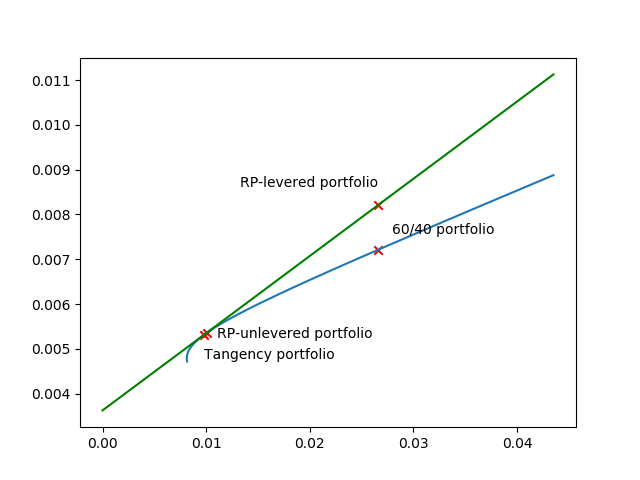
\includegraphics[scale=0.8]{figures/ex3.png}	
		\caption{RP-levered, RP-unlevered, Tangency, and 60/40 portfolio with efficient frontier}	
		\label{fig:ex3}
	
	\end{figure} 
	
	\textbf{What explains the difference between the RP and RP-unlevered portfolio performance?}
	
	\bigbreak	
	
	We now follow the same method but now by using the three-year monthly excess returns instead of the full sample. We obtain a mean of returns of the RP-unlevered portfolio using a rolling-window of $0.005280$ and a mean of returns of the RP-levered portfolio using a rolling-window of $0.007845$. These metrics are almost identical (slightly lower) than their full-window counterparts. \textbf{Why?}
	
	\bigbreak
	
	We now consider an investor who has a mean-variance utility U
	
	\begin{align*}
		U = \mu_{p} - \frac{a}{2}\sigma^{2}_{p}
	\end{align*}
	
	Using the full-sample estimates of the means and covariance matrix stocks and bonds, the optimal portfolio can be computed as follows:
	
	\begin{align*}
		w_{0} = \frac{1}{a} \Sigma^{-1} (\mu  - R_{0}\textbf{1})
	\end{align*}
	
	We end up with $42\%$ in stocks, $253\%$ in bonds and $-195\%$ in T-Bills. The metrics are the following
	
	\begin{table}[h!]
		\centering
 		\begin{tabular}{||c c||} 
 			\hline
 			& Metrics of optimal portfolio \\ [0.5ex] 
 			\hline\hline
 			mean & 0.008580 \\ 
 			std & 0.028735 \\
 			Sharpe ratio & 0.172410 \\ [1ex] 
 			\hline
		 \end{tabular}
	\end{table}	

\end{exercise}
  
\end{document}
